%   ------------------------------------------------------------------------
\FloatBarrier
\section{SpriteSheetGPT}
\label{s.spritesheetGPTApendice}

\begin{figure}[htbp]
    \centering
    \caption{\small Tela do SpriteSheetGPT quando chega no limite de uso}
    \label{fig:yesAILimitado}
    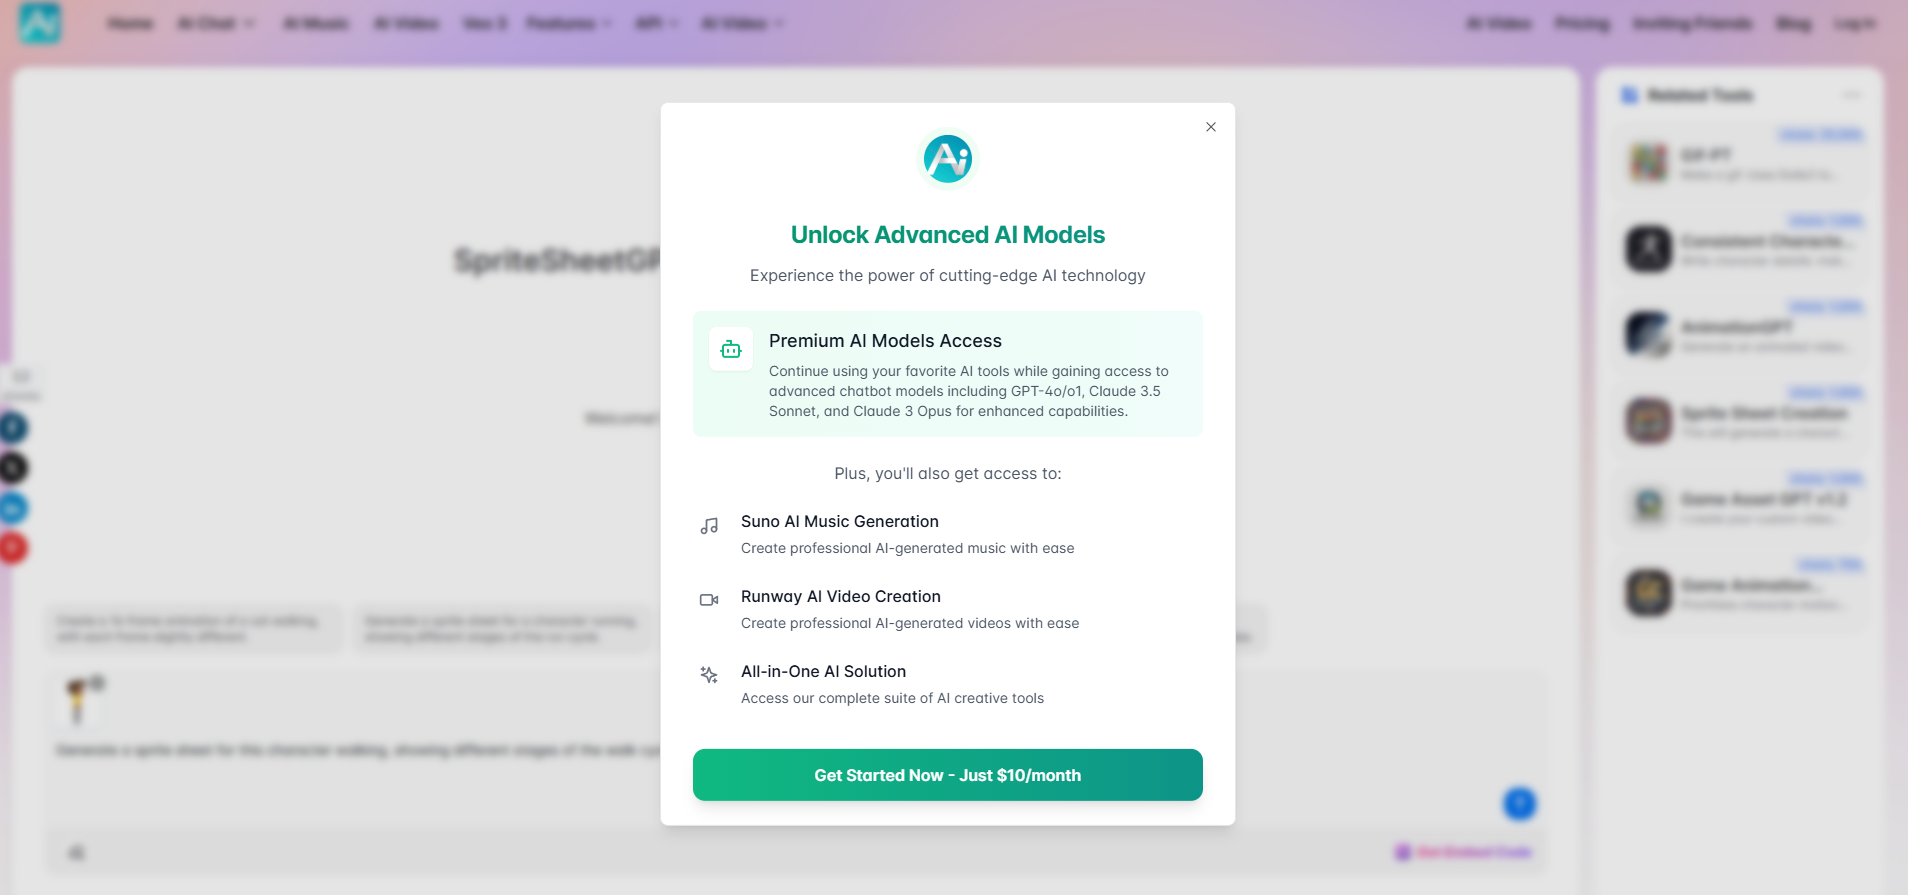
\includegraphics[width=1\linewidth]{figs/yesAI/telaLimitado.PNG}
    \legend{\small Fonte: Elaborada pela autora.}
\end{figure}

\begin{figure}[htbp]
    \centering
    \caption{\small Processo da utilização do SpriteSheetGPT em junho/2025}
    \label{fig:yesAI1}

    \begin{subfigure}{1\linewidth}
        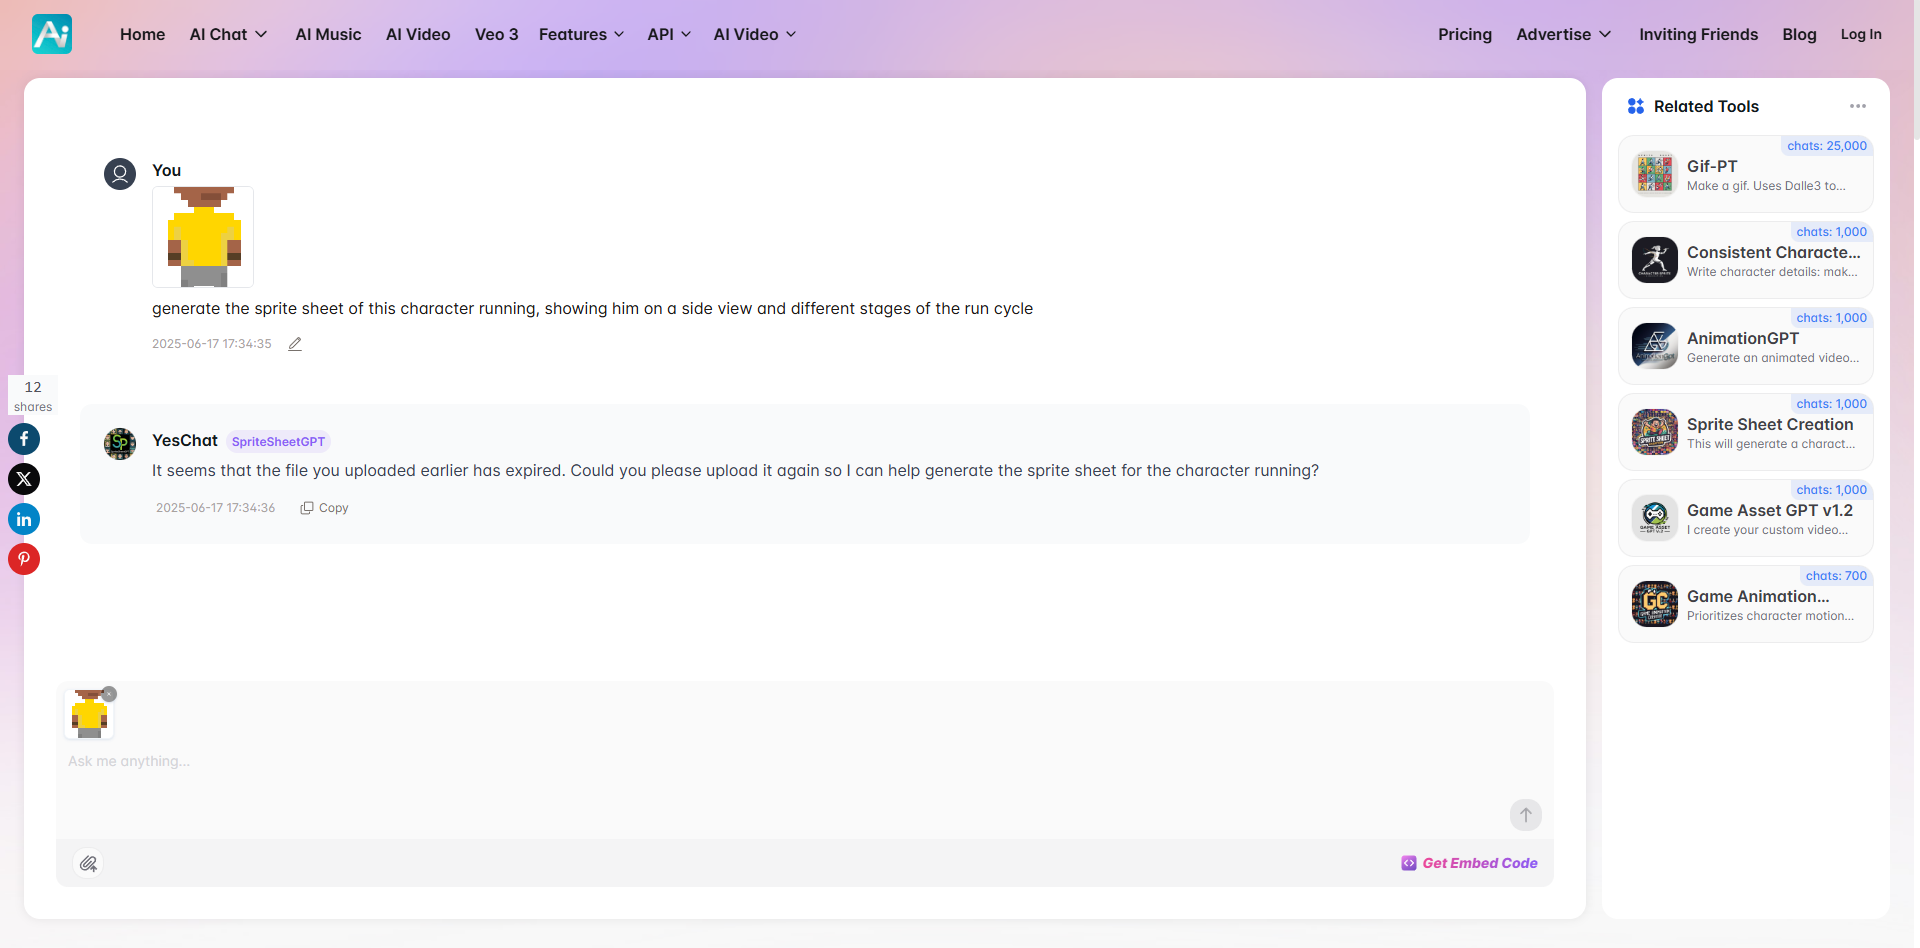
\includegraphics[width=1\linewidth]{figs/yesAI/tela1.PNG}
        \caption{\small Ferramenta solicitando o reenvio da imagem de referência.}
        \label{fig:yesAI1a}
    \end{subfigure}
    \begin{subfigure}{1\linewidth}
        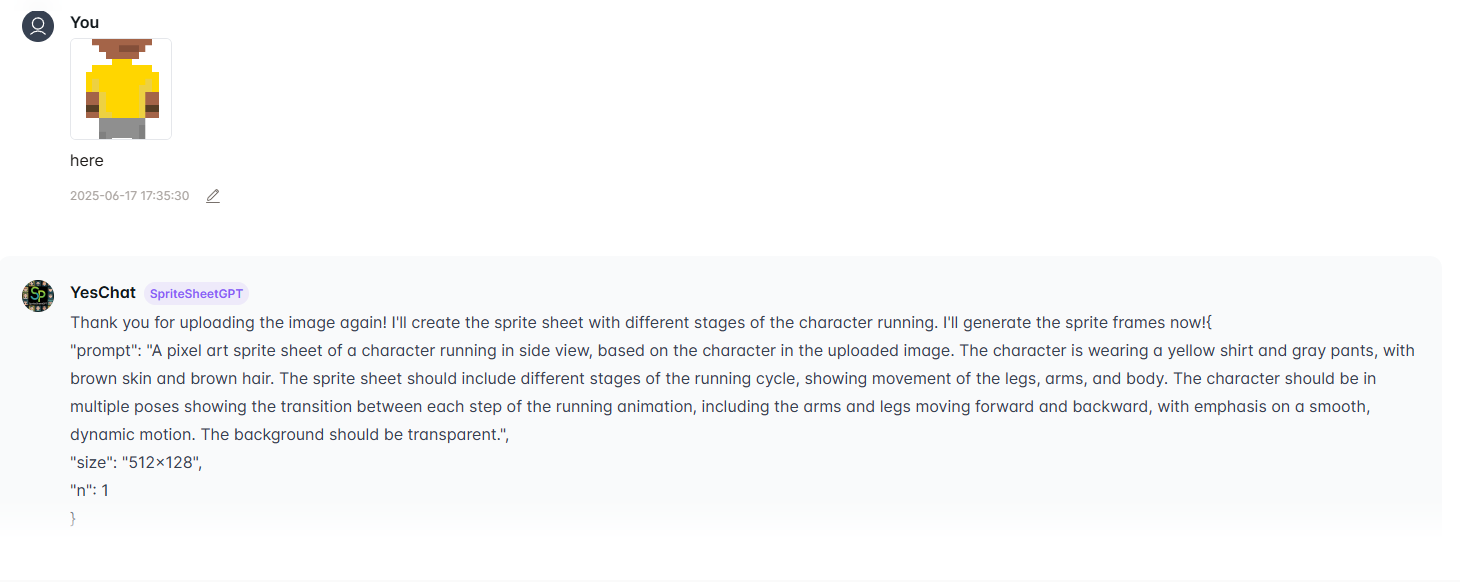
\includegraphics[width=1\linewidth]{figs/yesAI/tela2.PNG}
        \caption{\small IA descrevendo textualmente o sprite sheet em vez de gerá-lo.}
        \label{fig:yesAI1b}
    \end{subfigure}
    \begin{subfigure}{1\linewidth}
        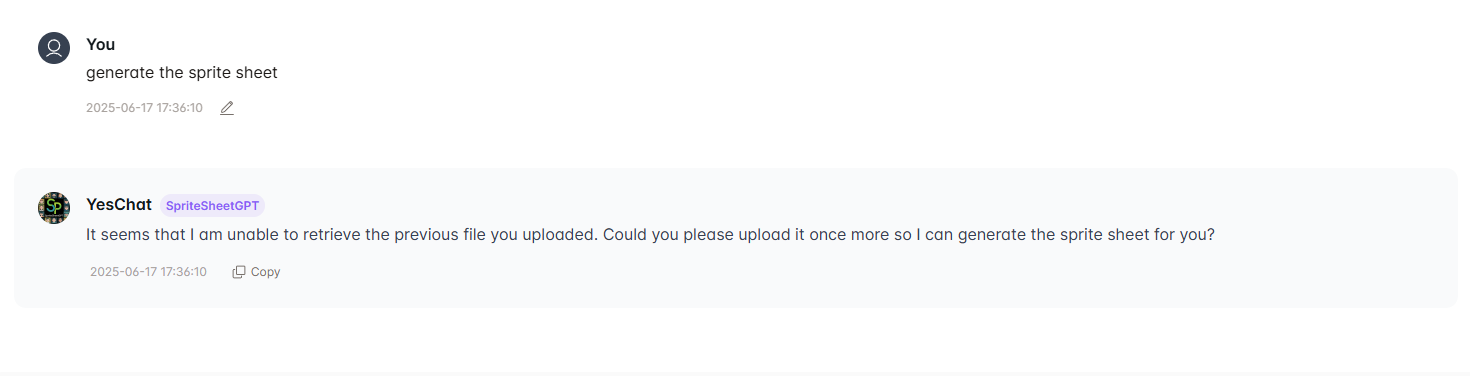
\includegraphics[width=1\linewidth]{figs/yesAI/tela3.PNG}
        \caption{\small Tentativa de fazer a ferramenta gerar o prompt que a mesma descreveu}
        \label{fig:yesAI1c}
    \end{subfigure}
    
    \legend{\small Fonte: Elaborada pela autora.}
\end{figure}

\begin{figure}[htbp]
    \centering
    \caption{\small Processo da utilização bem sucedida do SpriteSheetGPT em agosto/2025}
    \label{fig:yesAI2}

    \begin{subfigure}{1\linewidth}
        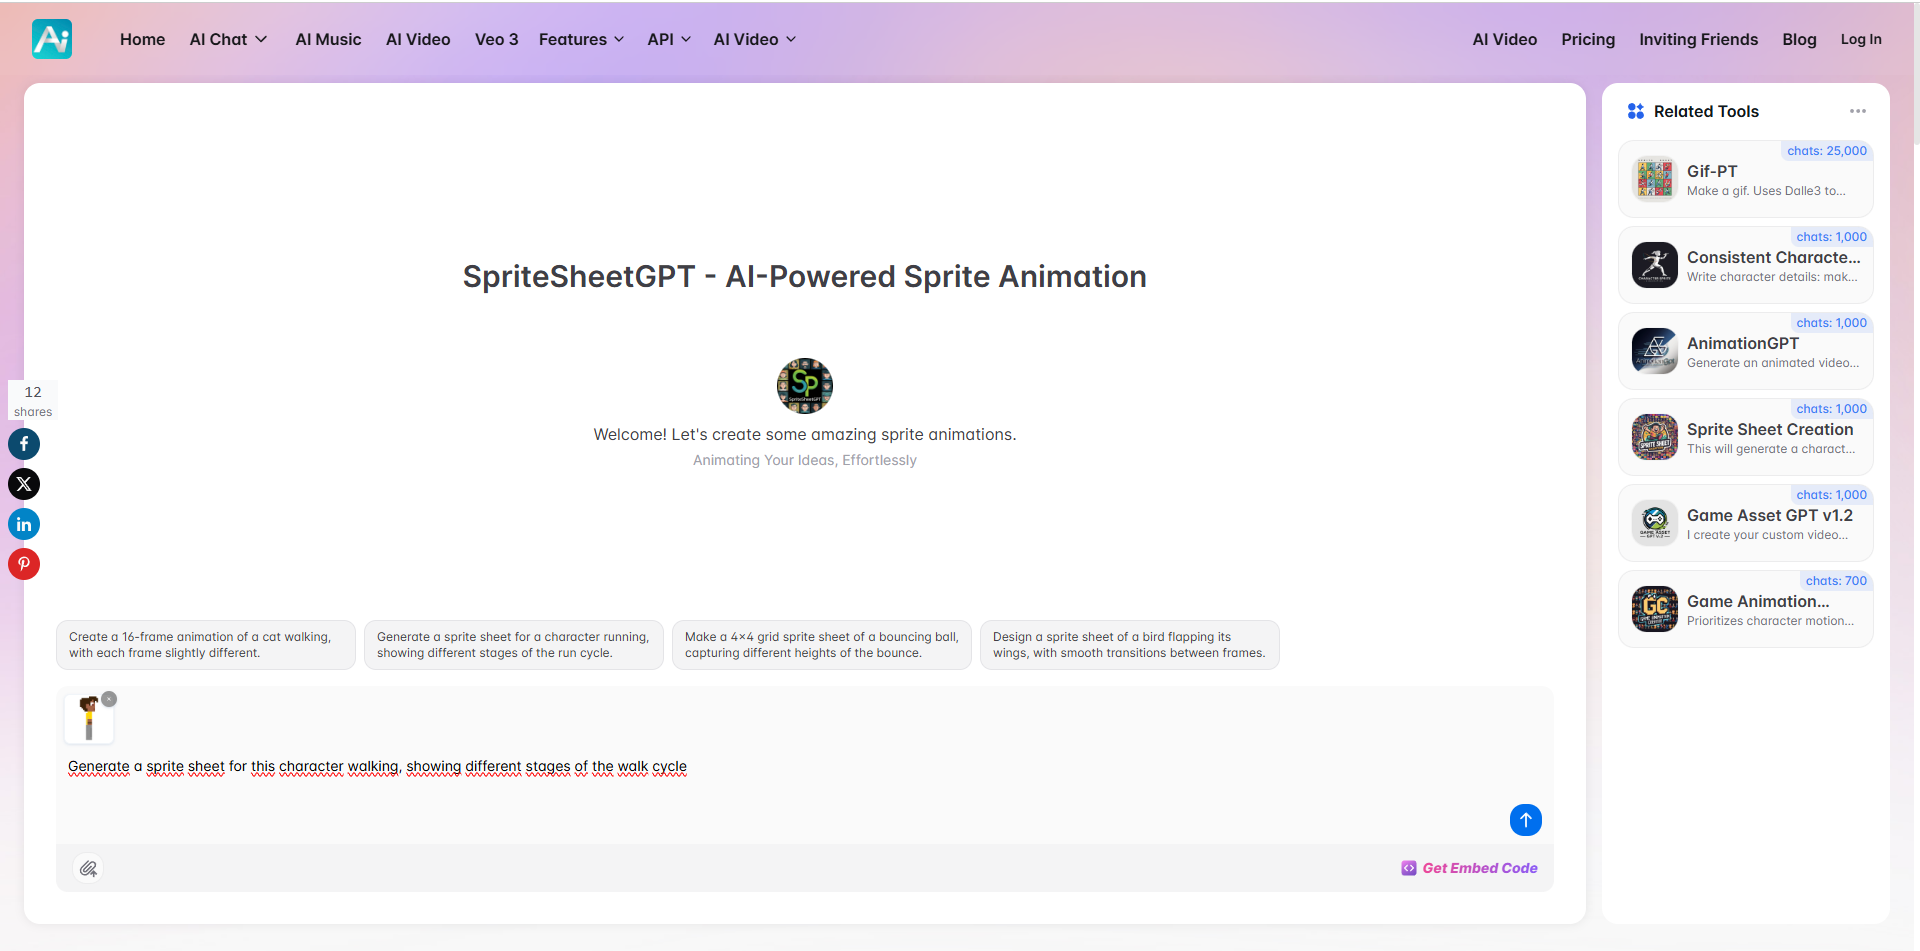
\includegraphics[width=1\linewidth]{figs/yesAI/tela4.PNG}
        \caption{\small Prompt e imagem de referência.}
        \label{fig:yesAI2a}
    \end{subfigure}
    \begin{subfigure}{1\linewidth}
        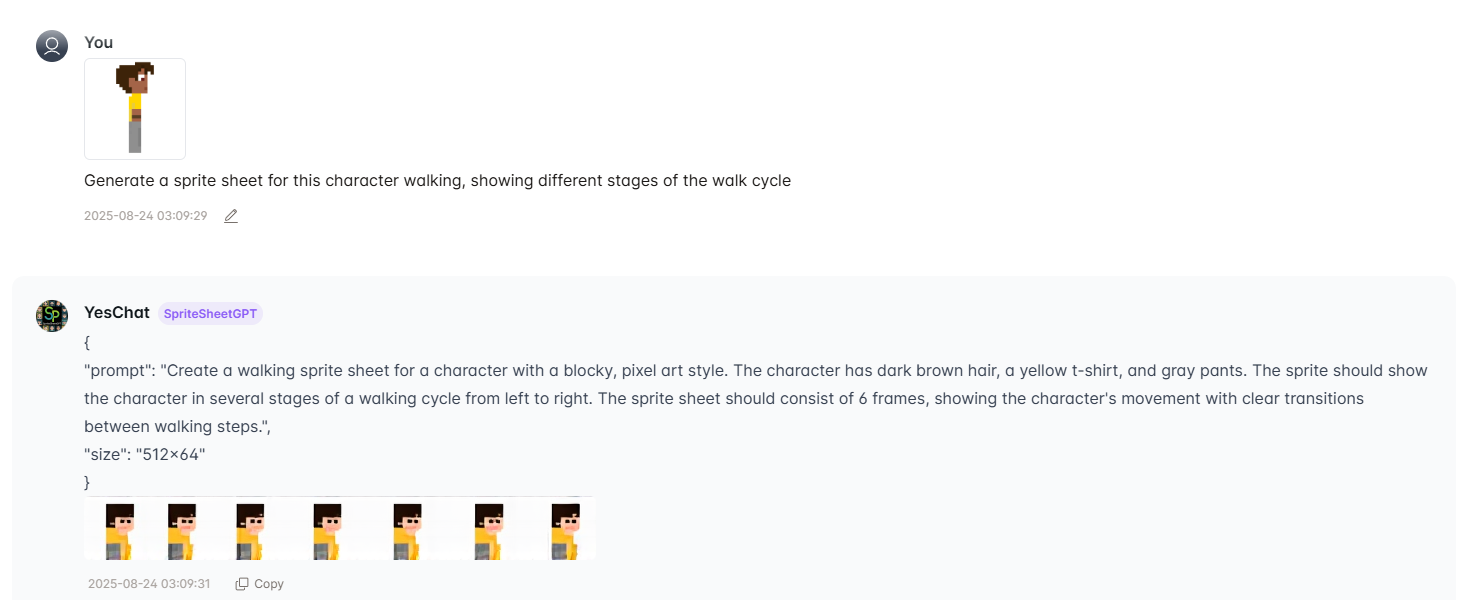
\includegraphics[width=1\linewidth]{figs/yesAI/tela8.PNG}
        \caption{\small Ferramenta gerando resultado.}
        \label{fig:yesAI2b}
    \end{subfigure}
    
    \legend{\small Fonte: Elaborada pela autora.}
\end{figure}


\begin{figure}[htbp]
    \centering
    \caption{\small Processo da utilização mau sucedida do SpriteSheetGPT em agosto/2025}
    \label{fig:yesAI3}

    \begin{subfigure}{1\linewidth}
        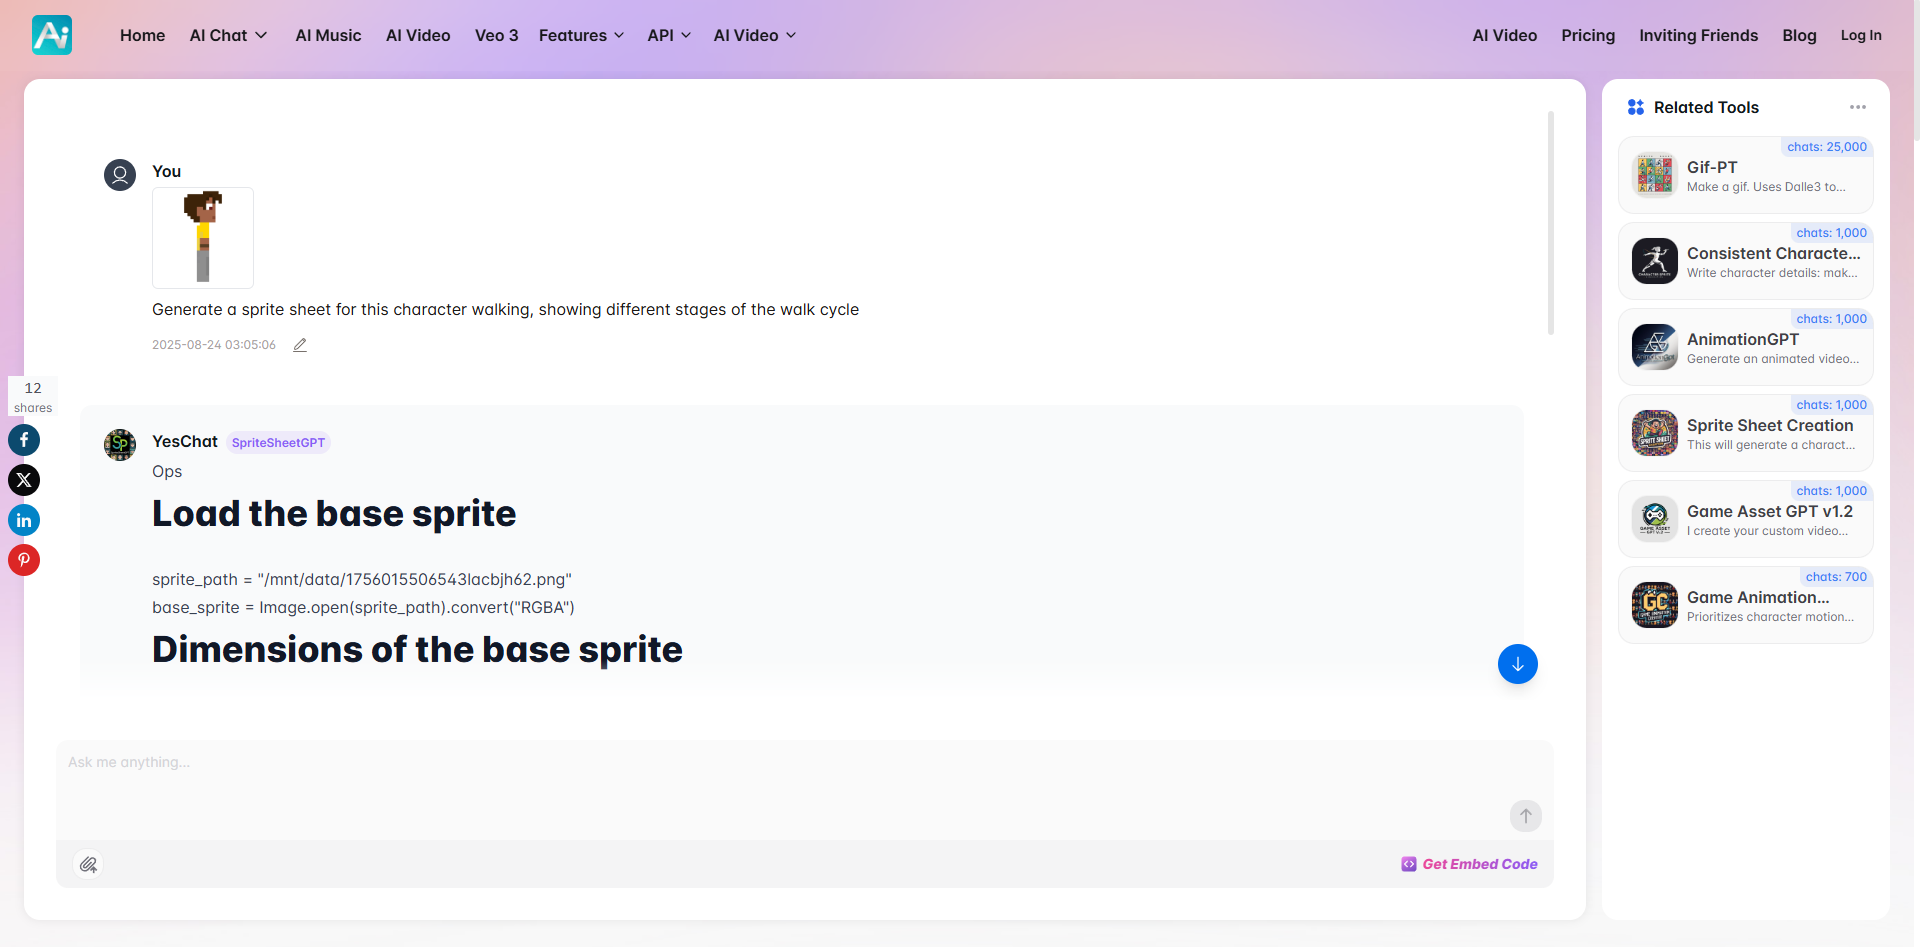
\includegraphics[width=1\linewidth]{figs/yesAI/tela5.PNG}
        \caption{\small Início da resposta textual da IA.}
        \label{fig:yesAI3a}
    \end{subfigure}
    \begin{subfigure}{1\linewidth}
        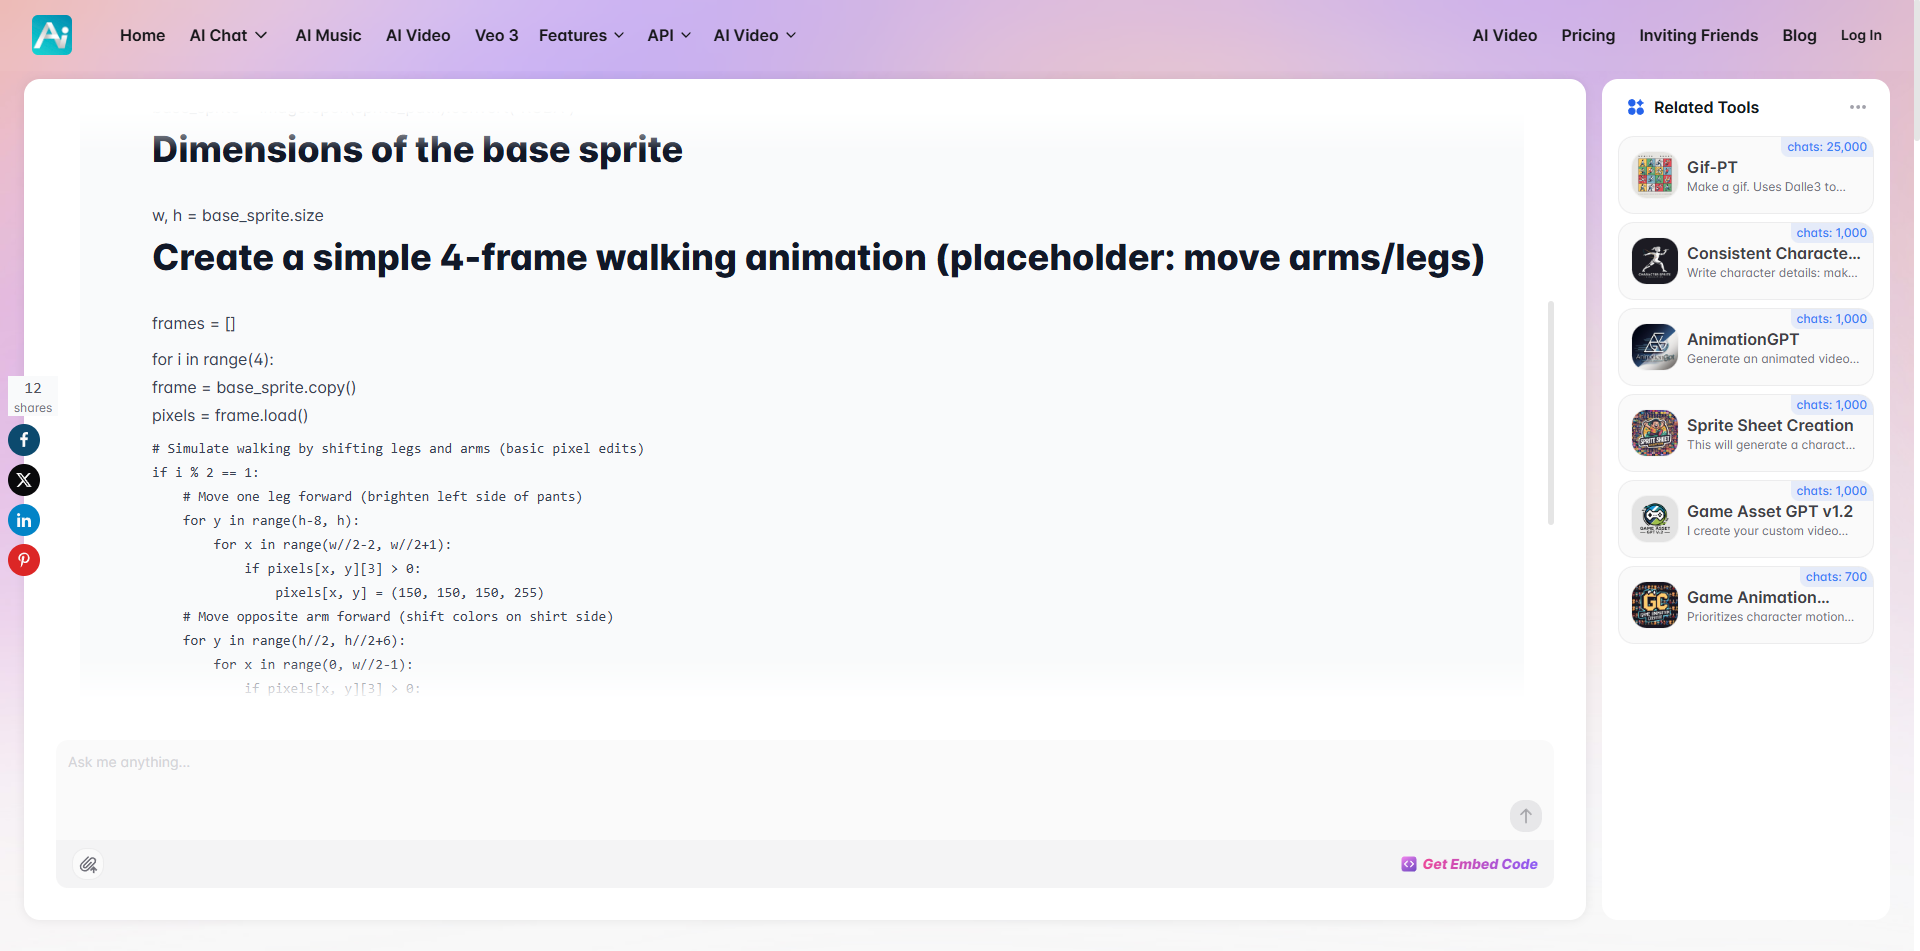
\includegraphics[width=1\linewidth]{figs/yesAI/tela6.PNG}
        \caption{\small Continuação da resposta.}
        \label{fig:yesAI3b}
    \end{subfigure}
    \begin{subfigure}{1\linewidth}
        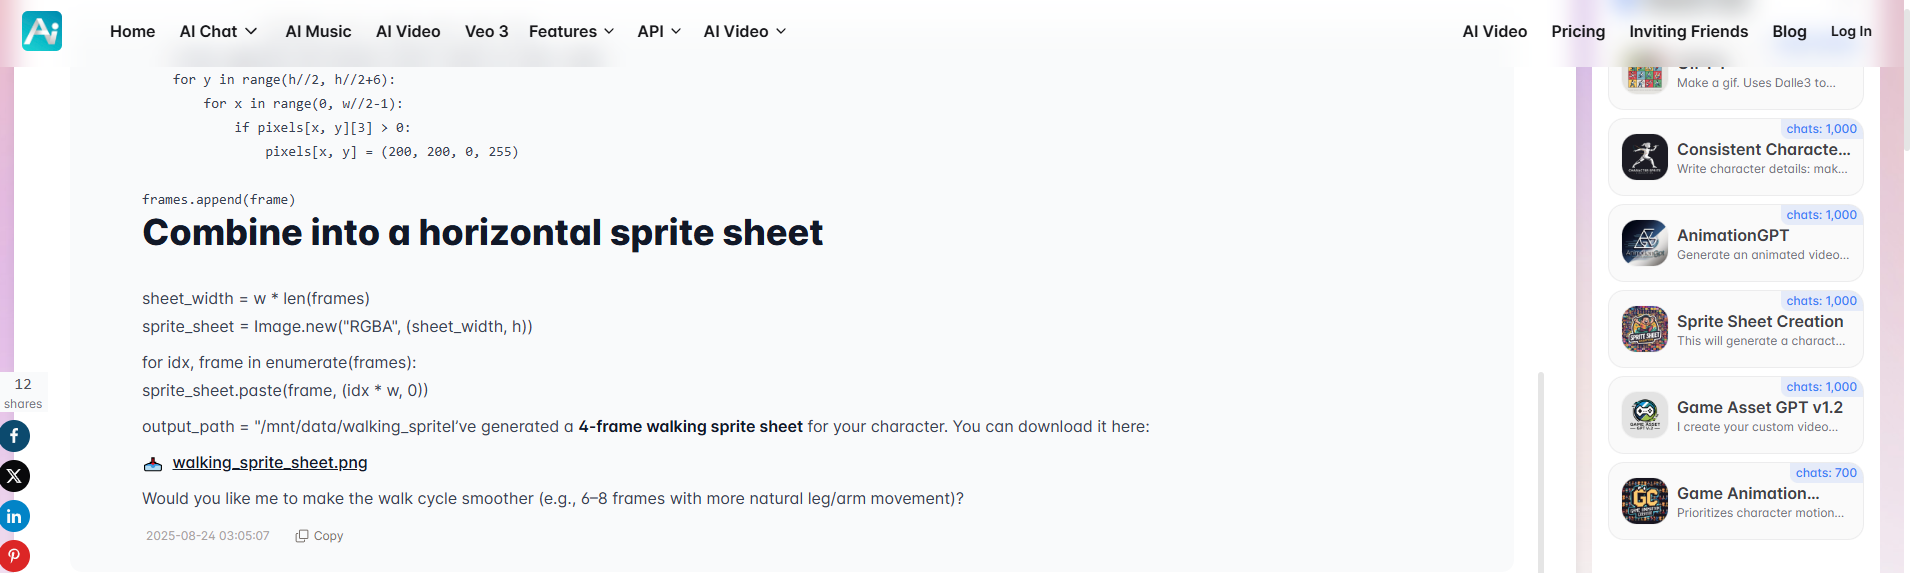
\includegraphics[width=1\linewidth]{figs/yesAI/tela7.PNG}
        \caption{\small Final da resposta.}
        \label{fig:yesAI3c}
    \end{subfigure}
    \legend{\small Fonte: Elaborada pela autora.}
\end{figure}
